\documentclass[a4paper,12pt]{article}
\usepackage[utf8]{inputenc}
\usepackage[french]{babel}
\usepackage[T1]{fontenc}
\usepackage[top=2cm,bottom=2cm,left=2cm,right=2cm]{geometry}
\usepackage{graphicx}
\usepackage{wrapfig}
\usepackage{url}

\begin{document}

\begin{titlepage}
	\begin{center}
		\Large{Année universitaire 2016-2017}\\
		\Large{Université de Caen Basse-Normandie}\\[1cm]
		
		\huge{Rapport sur la création et la gestion des thèmes, du style et de l'apparence globale de l'IDE}\\
		\vspace{3cm}
		
		Thomas Lécluse
		
	\normalsize{\textit{ ~ L2 Informatique}}\\
		\medskip
		\vspace{2cm}
		
	\end{center}
\end{titlepage}

\tableofcontents
\newpage

\section{Les thèmes}
	
	Afin de pouvoir rendre plus personnalisable l'application, nous avons choisi de permettre la personnalisation du thème global.
	Voici quelques exemples de thèmes : 
	
	
		\begin{figure}[h!]
			\begin{center}
				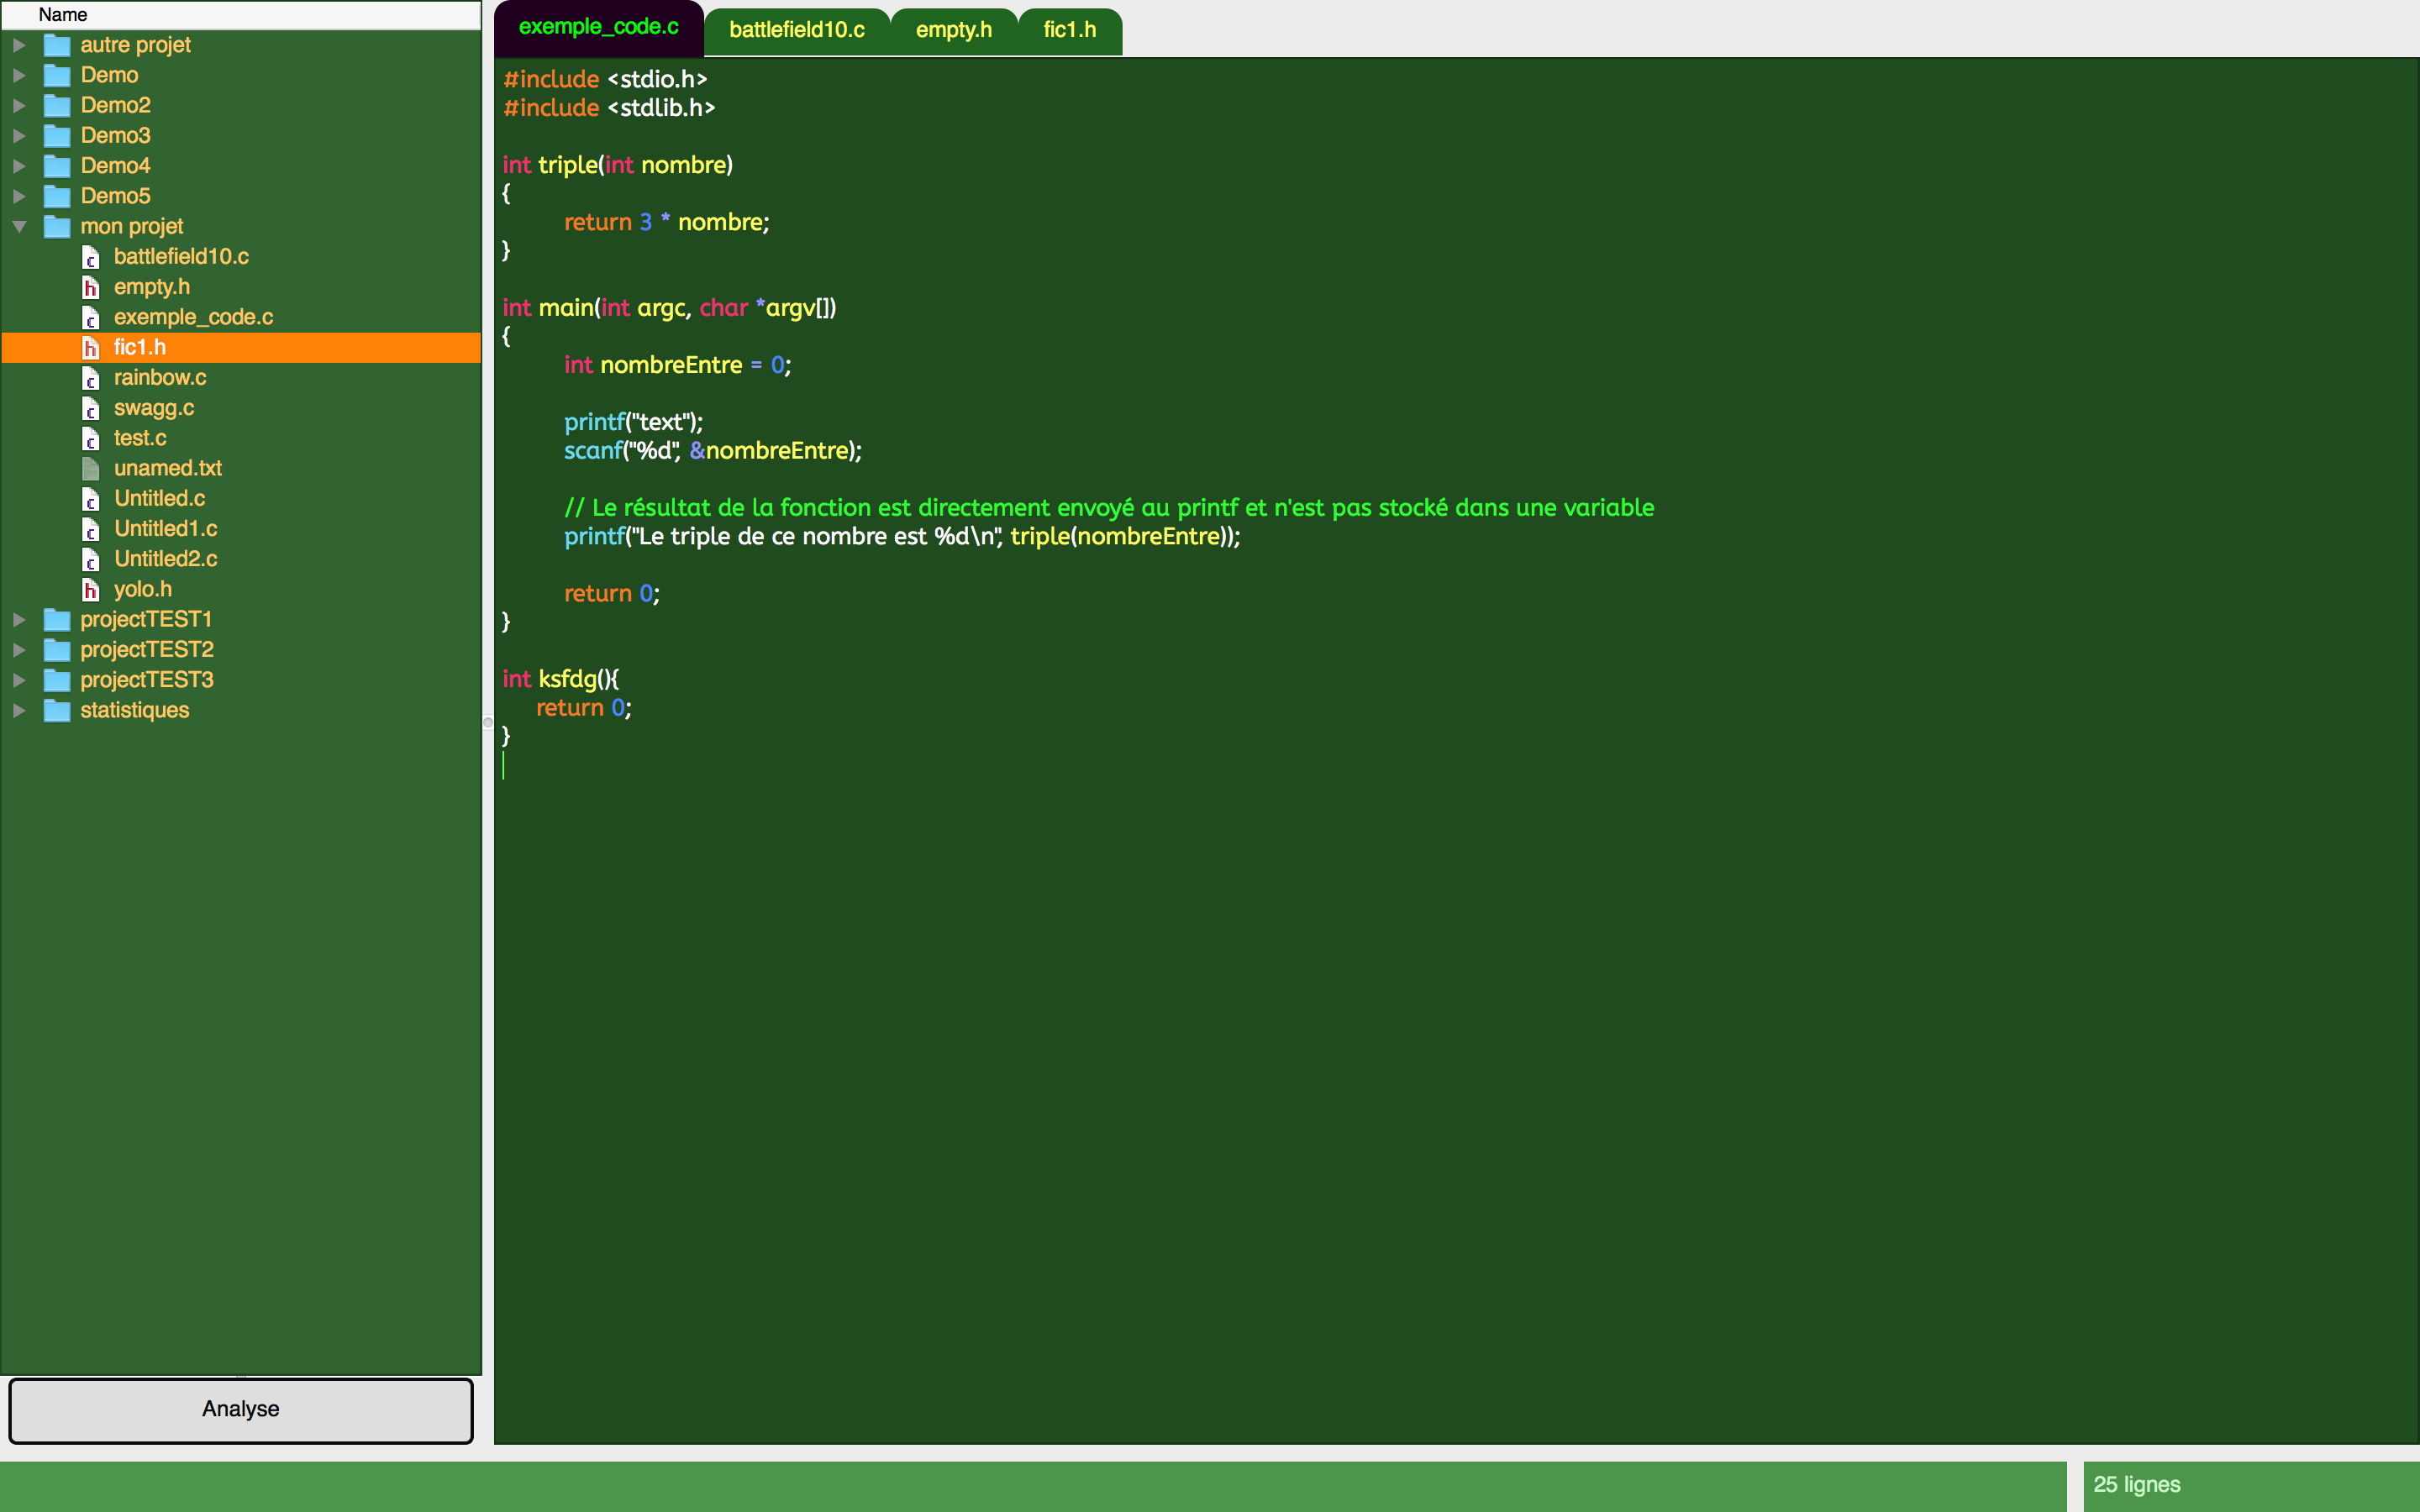
\includegraphics[scale=0.17]{imgs/theme_forest}
				\caption{Thème Forêt}
			\end{center}
		\end{figure}
		
		\begin{figure}[h!]
			\begin{center}
				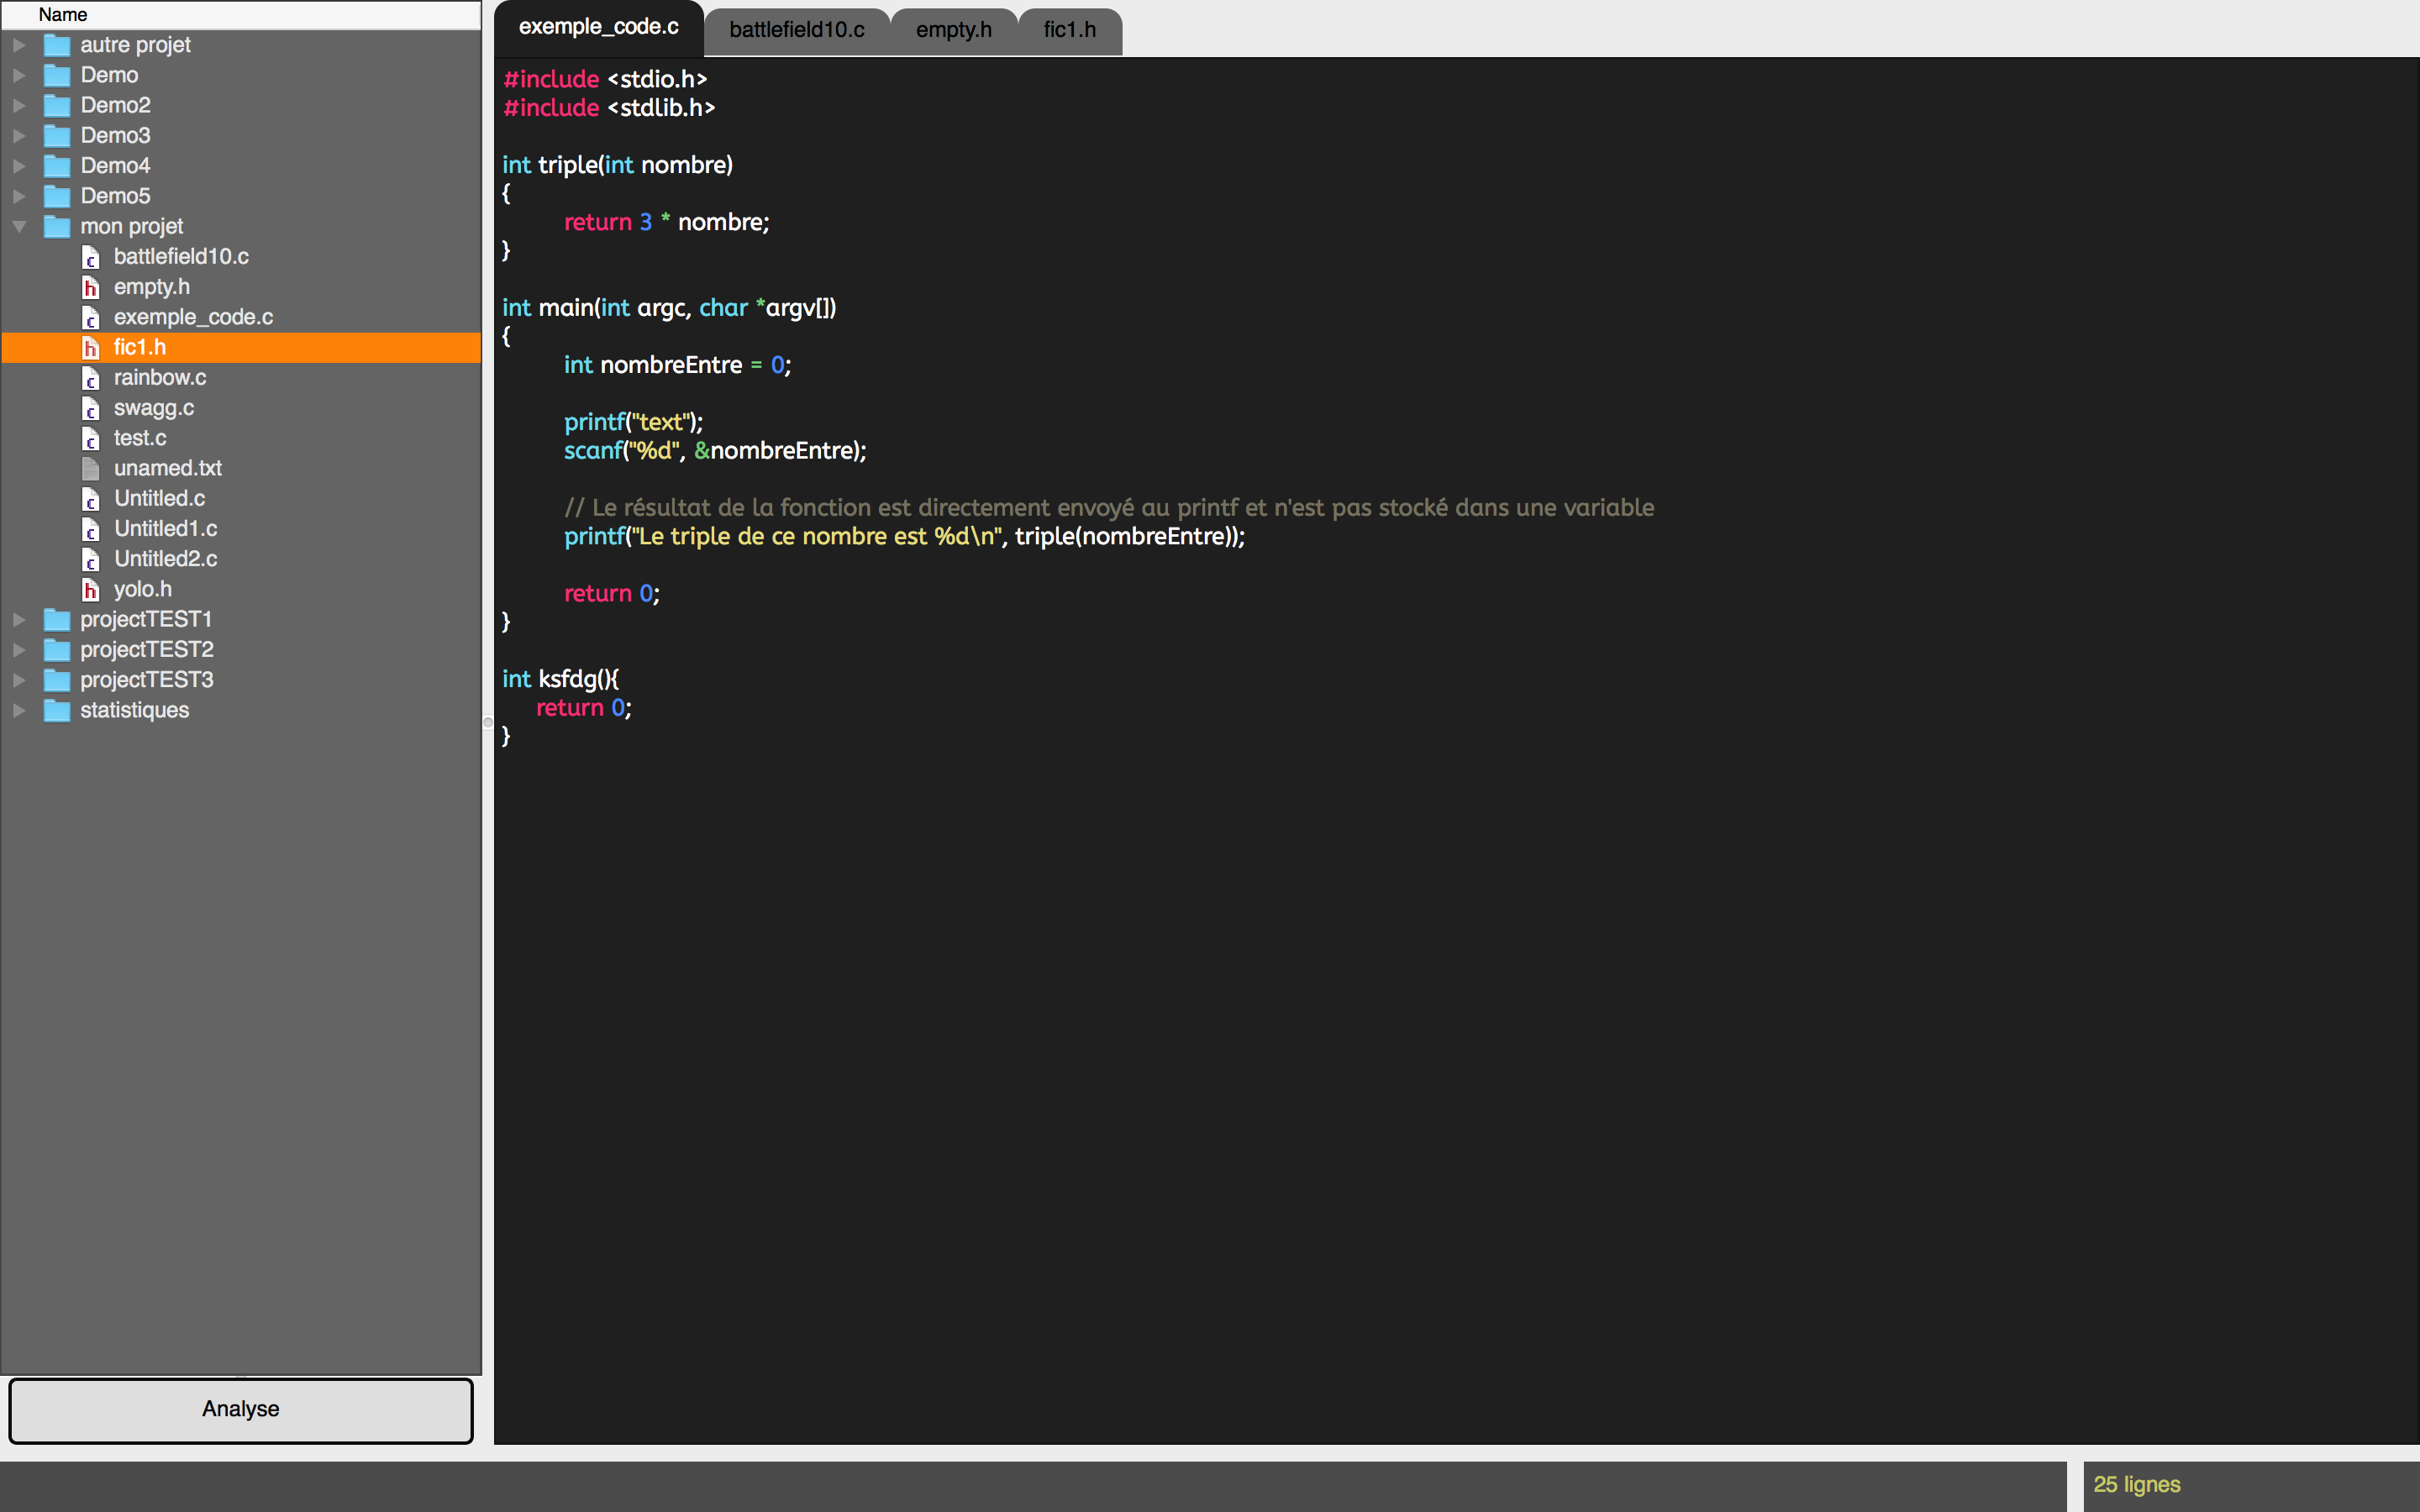
\includegraphics[scale=0.17]{imgs/theme_basic}
				\caption{Thème de base}
			\end{center}
		\end{figure}
		
		\begin{figure}[h!]
			\begin{center}
				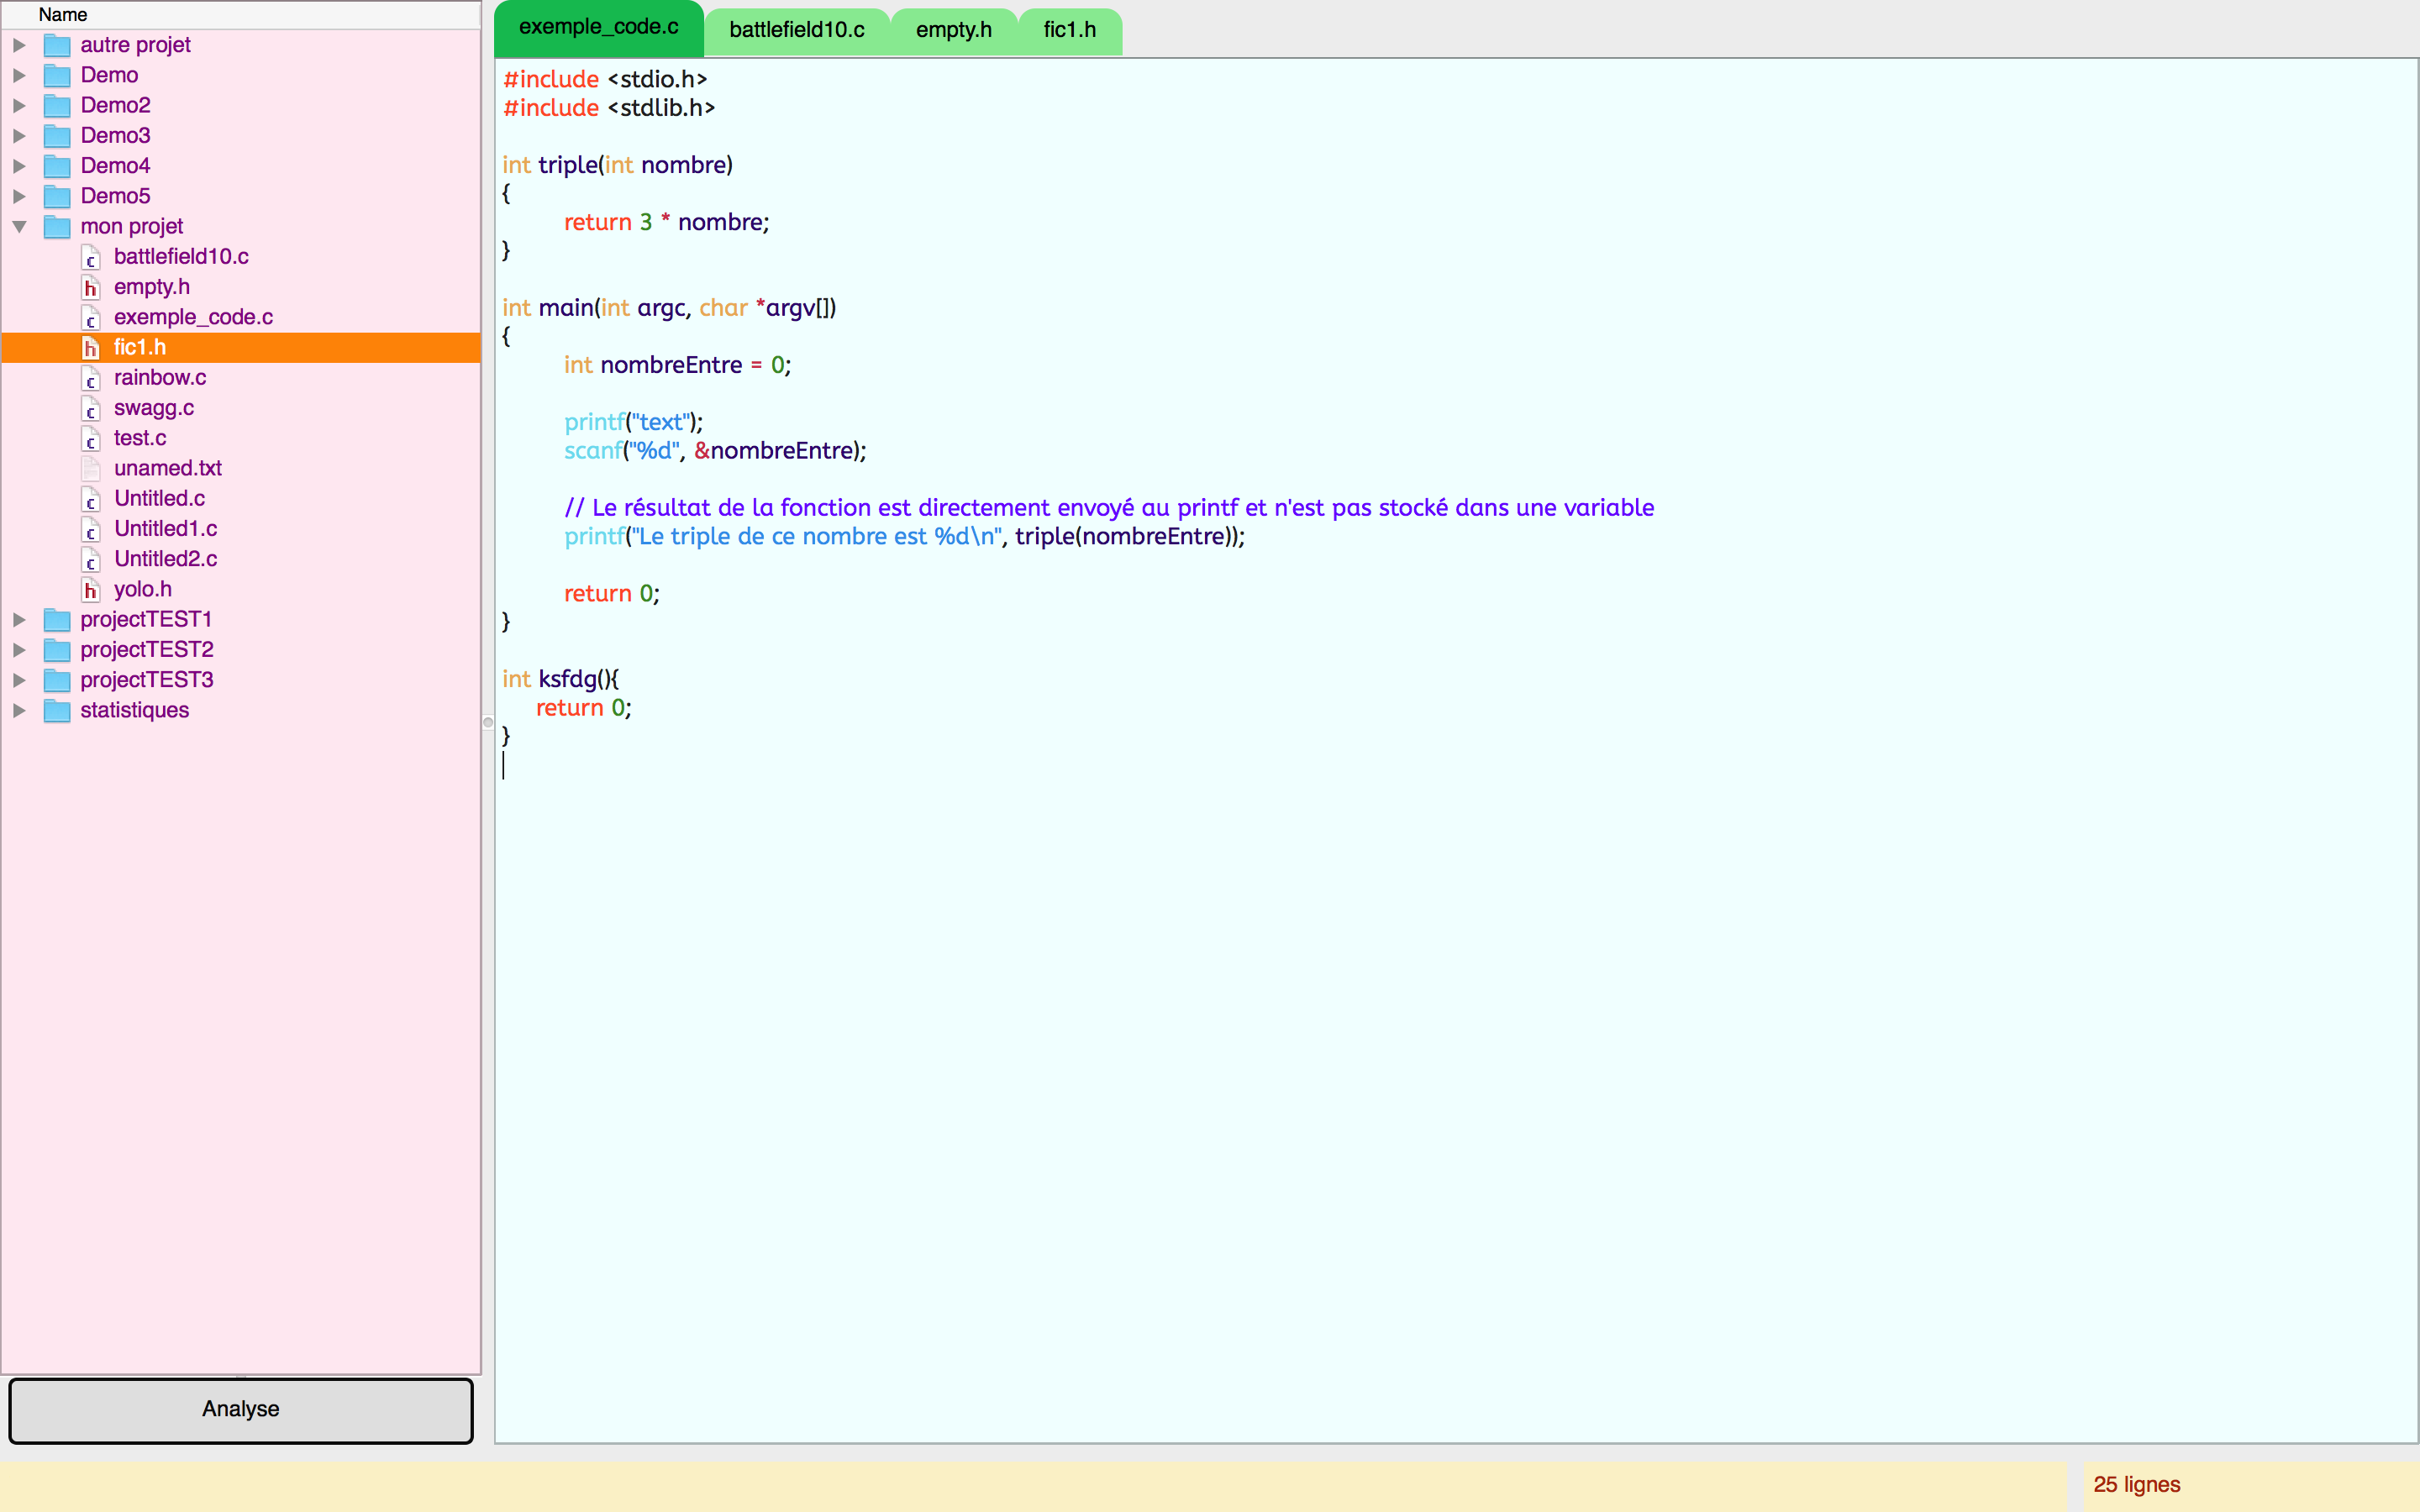
\includegraphics[scale=0.17]{imgs/theme_pastel}
				\caption{Thème Pastel}
			\end{center}
		\end{figure}
		
		\subsection{Changer de thème}
		
			Le changement de thème est très simple. Il suffit de se rendre dans le menu "apparence" puis de choisir son thème parmi ceux proposés.
	
			\begin{figure}[h!]
				\begin{center}
					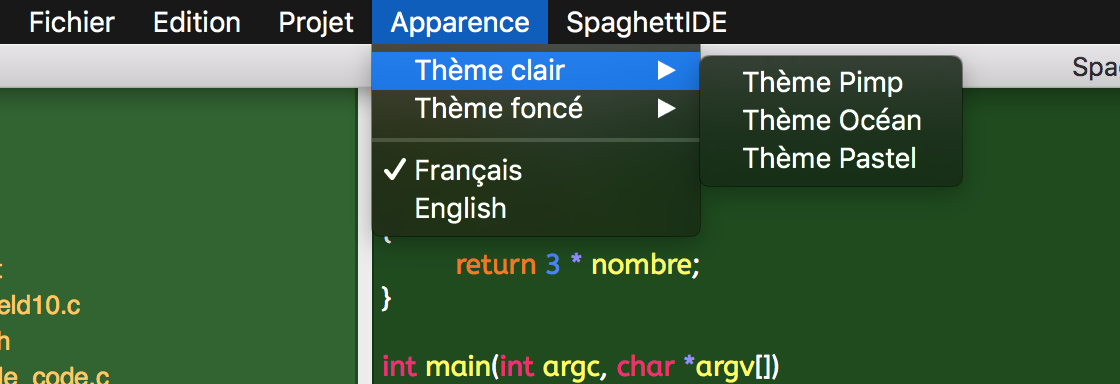
\includegraphics[scale=0.7]{imgs/choix_theme}
					\caption{Choix de son thème}
				\end{center}
			\end{figure}
			
			Les thèmes sont triés en fonction de si ils sont plutôt clairs ou plutôt sombres.\\
			Lorsque l'on sélectionne son thème il est immédiatement changé, il n'y a pas besoin de relancer l'application. De plus, une petite icone apparaît à côté du thème que vous avez choisi dans la barre de menu\\
			
			De plus lorsque vous relancerez l'IDE, le dernier thème que vous avez utilisé sera rechargé.
			
		\subsection{Gestion des thèmes}
		
			Les thèmes sont regroupés dans des répertoires distincts, le tout dans le répertoire "theme" situé à la racine du projet. 
			\begin{figure}[h!]
				\begin{center}
					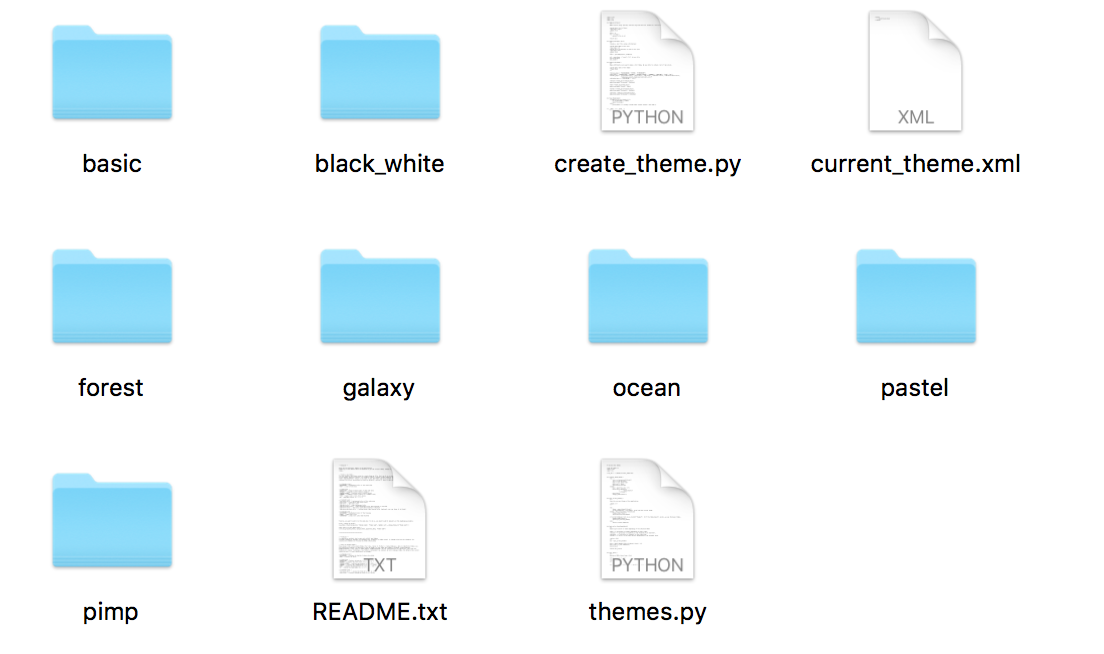
\includegraphics[scale=0.7]{imgs/themes}
					\caption{Contenu du répertoire "theme"}
				\end{center}
			\end{figure}
			
			Chaque répertoire de thème regroupe les fichiers en format .json. Les différents fichiers .json contiennent les couleurs en RGB d'un élément de l'interface graphique.
			
			\begin{figure}[h!]
				\begin{center}
					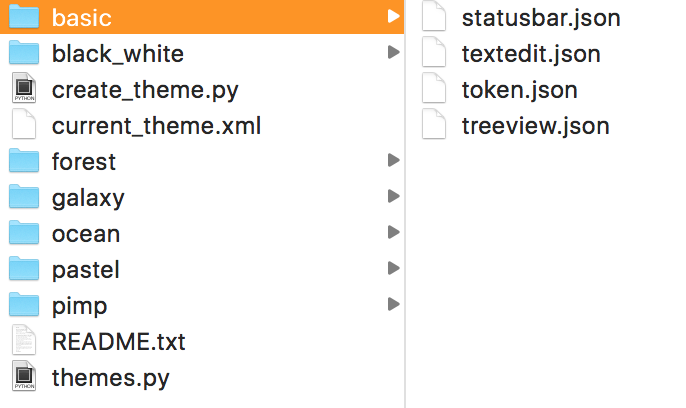
\includegraphics[scale=0.7]{imgs/basic_json}
					\caption{Contenu du répertoire "basic" (le contenu est semblable pour tous les thèmes)}
				\end{center}
			\end{figure}
			\begin{figure}[h!]
				\begin{center}
					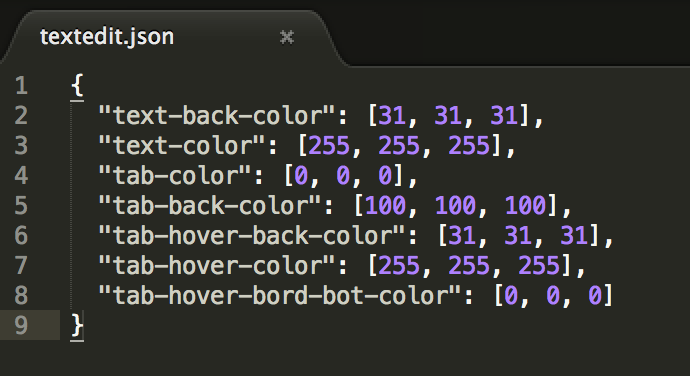
\includegraphics[scale=0.7]{imgs/exemple_json}
					\caption{Exemple de fichier .json pour les thèmes.}
				\end{center}
			\end{figure}
			
			Le module theme.py nous permet de récupérer le thème sauvegardé (dans le fichier currenttheme.xml) lors du chargement de l'application notament. Ici sont également contenues les méthodes permettant à l'interface d'aller chercher les couleurs qu'elle doit appliquer aux différents éléments.\\
			
			Au niveau technique, nous utilisons la méthode .setStyleSheet() de QT qui peut s'appliquer à la majorité des widgets (tous dans notre cas) et qui nous permet donc de spécifier et de modifier les couleusr de fond ainsi que de police des widgets en fonction du thème choisi.
			
		\subsection{Création de thèmes}
		
			Vous pouvez utiliser les thèmes pré-définis, qui ont été pour la plupart validés et certifiés par la totalité du groupe comme étant jolis, mais vous pouvez aussi créer vos propres thèmes.\\
			
			Le script "createtheme.py" vous permet cela, et la démarche à suivre est expliquée dans le fichier README.txt.\\
			
			Pour résumer, on lance le fichier createtheme.py via un terminal en spécifiant le nom du thème. Tapez par exemple :
			"python3 createtheme.py monNouveauTheme" et cela créera un répertoire "monNouveauTheme" qui contiendra les fichiers nécessaires à la gestion de votre thème. Ouvrez ensuite les fichiers .json et définissez vos propres couleurs (par défaut tout est noir).\\
			
			Une fois cela fait, vous devrait ajouter deux lignes dans le module menu.py pour que votre thème apparaisse dans la séléction.

			\begin{figure}[h!]
				\begin{center}
					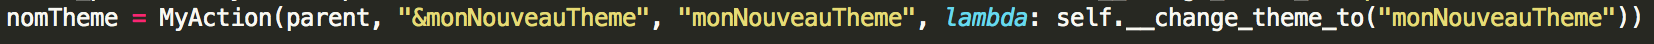
\includegraphics[scale=0.5]{imgs/add2}
					\caption{Où nomTheme est le nom de la variable pour le thème, et monNouveauTheme le nom que vous avez donné à votre thème}
				\end{center}
			\end{figure}
			\begin{figure}[h!]
				\begin{center}
					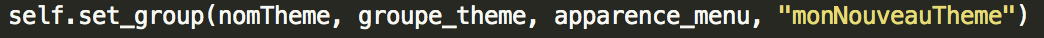
\includegraphics[scale=0.7]{imgs/add1}
					\caption{Où nomTheme est le nom de la variable pour le thème, et groupetheme le groupe (clair ou sombre) auquel appartient votre thème}
				\end{center}
			\end{figure}
			
			Votre thème apparaît maintenant dans la barre de menu et il est sélectionnable !
			
	\section{Les langues}
	
		Comme vous avez pu le remarquer précédemment dans le menu "apparence", juste sous les thèmes il y a le choix de la langue, français ou anglais (pour le moment).\\
		
		Actuellement ces fonctions ne sont reliées à rien, mais la langue pourra être modifiée par la suite.
		Pour faire cela nous consacrerons un module contenant un ou plusieurs dictionnaires qui donneront en fonction de la langue actuelle, le texte dans la langue correspondante. 

	\section{Ajout sur l'interface}
	
		Nous avons également travaillé à étoffer l'interface. Nous avons rajouté une seconde barre de status (en bas à droite), servant à afficher des informations sur le code lui-même :
		
		\begin{figure}[h!]
			\begin{center}
				
\includegraphics[scale=1]{imgs/nb_lignes}
				\caption{Le nombre de lignes du fichier courant}
			\end{center}
		\end{figure}
		\begin{figure}[h!]
			\begin{center}
				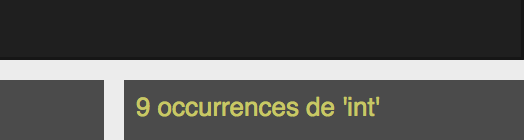
\includegraphics[scale=1]{imgs/nb_occu}
				\caption{Le nombre d'occurences d'une recherche effectuée}
			\end{center}
		\end{figure}
		
		Nous utilisons de plus cet emplacement (en bas à droite) pour afficher une barre de status qui sert pour le moment uniquement à indiquer la progression lors du chargement de projet (Yacc lisant tous les fichiers afin de récupérer les différentes fonctions à travers les modules, cela peut prendre plusieurs secondes).
		\begin{figure}[h!]
			\begin{center}
				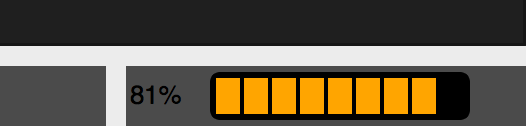
\includegraphics[scale=1]{imgs/progress}
				\caption{Barre de progression lors du chargement d'un projet de l'utilisateur}
			\end{center}
		\end{figure}
		
		Le style appliqué à la progressBar n'étant pas relatif au thème, et différent de celui de base, il est géré dans un module dédié (c.f section ci-dessous sur le style externe)
		
		\subsection*{Quelques problèmes}
		
			Nous avons rencontré des problèmes lors de l'affichage et l'actualisation de la barre de status.\\
			
			En effet, le traitement effectué par Yacc doit être effectué en parallèle du processus principal (où tourne l'application) afin de pouvoir actualiser la valeur de la barre de progression. Nous utilisons pour le moment un Thread qui effectue le calcul de Yacc, puis un autre qui actualise la barre de status car celle-ci doit lire en continue le valeur d'une variable l'actualiser si elle a été modifiée.\\
			 Si on fait l'actualisation de la barre de status dans le processus principal, l'interface est bloqué et la barre n'est pas actualisée.
			 
			 Le problème est que : sur une autre machine qu'un Mac, le serveur graphique plante et l'application avec. Seul le Mac semble suporter la modification de la barre de status depuis un Thread...\\
			 Pour le moment, en fonction du système d'exploitation, nous effectuons le traitement de Yacc soit dans un Thread si on a un Mac, soit dans le processus principal si on a autre chose, mais dans ce cas, la barre de status n'est pas actualisée.
			 
			\subsection*{Résolution}
			
			Nous sommes parfaitement consients que le projet doit fonctionner aussi bien sur Linux que sur Mac et c'est pourquoi nous recherchons activement des solutions.\\
			
			Nous avons deux idées pour le moment :
			\begin{itemize}
				\item Utiliser un QTimer de QT qui va appeler une fonction régulièrement, cela utilise un Thread, mais c'est plus léger qu'un Thread, il y a donc des chances que ça fonctionne
				
				\item Utiliser le multiprocessing python, on ne sait pour le moment pas trop comment ça fonctionne, mais ça permet de lancer plusieurs processus en parallèle sans pour autant utiliser des Threads. Ça pourrait être donc une autre idée. 
			\end{itemize}
		
	\section{Style externe}
	
		Dans le répertoire gui qui contient tout ce qui est relatif à l'interface graphique, il y a un répertoire style qui regroupe des éléments auxquels on applique également des feuilles de styles (via la méthode setStyleSheet() des widgets dans QT; de même que pour les thèmes).
		\begin{figure}[h!]
			\begin{center}
				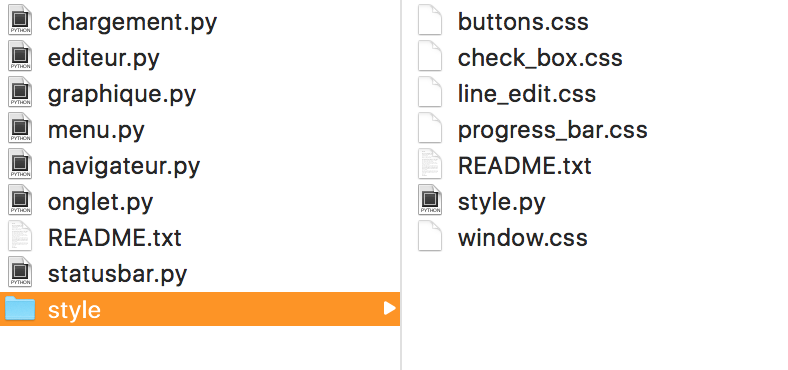
\includegraphics[scale=1]{imgs/style}
				\caption{Contenu du répertoire style}
			\end{center}
		\end{figure}
				
		Chaque document .css contient le style relatif à des éléments. Nous retrouvons ici le style appliqué :
		
		\begin{itemize}
			\item aux boites de dialogue
				\begin{figure}[h!]
					\begin{center}
						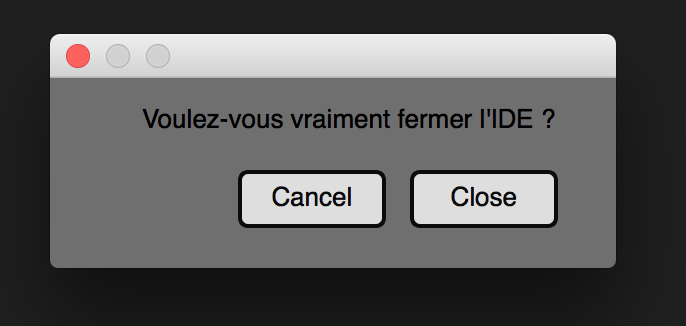
\includegraphics[scale=0.4]{imgs/quit}
						\caption{ Exemple de la fermeture de l'IDE : une popup qui apparaît demandant la confirmation.}
					\end{center}
				\end{figure}
				
			\item aux boutons, à qui on inverse les couleurs lorsqu'on les survole
				\begin{figure}[h!]
					\begin{center}
						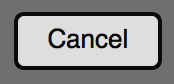
\includegraphics[scale=1]{imgs/bout1}
						\caption{Style appliqué à un bouton normal.}
					\end{center}
				\end{figure}
				\begin{figure}[h!]
					\begin{center}
						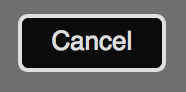
\includegraphics[scale=1]{imgs/bout2}
						\caption{Le même bouton lorsqu'il est survolé par la souris.}
					\end{center}
				\end{figure}
				
			\item à la barre de status
			\begin{figure}[h!]
					\begin{center}
						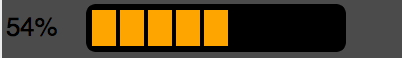
\includegraphics[scale=0.7]{imgs/progress2}
						\caption{La barre de status vue ci-dessus.}
					\end{center}
				\end{figure}
		\end{itemize}
		
\end{document}